\documentclass[pdftex,10pt]{article}
\usepackage{fullpage}
\usepackage{graphicx}
\usepackage{natbib}
\usepackage{amsmath}

\title{Storm Surges}

\date{\today}

\begin{document}
\maketitle

\begin{abstract}
Abstract to be completed
\end{abstract}

\section{Introduction}\label{sec:intro}


%some general intro paragraph here

%my attempt at physical oceanopgraphy SoG- Susan feel free to edit.
The Strait of Georgia is a strongly stratified, semi-enclosed body of water located between Vancouver Island and the mainland of British Columbia. It is part of a larger system of waterways collectively known as the Salish Sea and is connected to the Pacific Ocean via the Strait of Juan de Fuca and Johnstone Strait. Several features related to the physical oceanopgraphy of this region render it difficut to model numerically. The outlfow from the Fraser River in the late spring is the primary source fresh water within the Strait of Georgia, and leads to large density gradients in the summer months. Additionally, strong tidal mixing through the San Juan and Gulf Islands produces horizontal density gradients that separate the saline waters of the Strait of Juan de Fuca and the fresher water of the Strait of Georgia. It is important to accurately represent the vertical mixing in this region as it sets the rate of export of fresh water through estuarine circulation. The strong and fast tidal currents through the narrow channels of the north, such as Discovery Passage and Johnstone Strait, pose a particular challenge for numerical models. Yet, several modelling efforts for this region exist, ranging in choices of grid structure, mixing parametrizations, and domain size and extent. 

%overview oF SoG/Salish Sea models


%intro to storm surges
Many coastal communities in the Strait of Georgia are at risk to flooding and property damaged caused by storm surges, a natural hazard arising from the combination of a strong storm and high tide. The low atmospheric pressure associated with a storm acts as an inverse barometer elevating the sea level. This effect in combination with strong winds pushing water up against the coast can cause flooding, particularly if the storm occurs during an unusually high tide.  Additionally, there is a small contribution to increased sea level due to the thermal expansion of water during warmer years set by the El Nino Southern Oscillation (ENSO) \citep{abeys2011extreme}. %more on past events, significance

%storm surge modelling

%overview of paper: model configuration, model evaluation, storm surge hindcasts.

\section{Model Configuration}\label{sec:config}
%To be included: NEMO overview, tides, rivers, bathymetry, atmospheric forcing, vertical/lateral mixing, boundary conditions, grid. 

%A section about how we configured the model for SoG 
We have used the Nucleus for European Modelling of the Ocean (NEMO) framework in its regional configuration to develop an ocean model for the Strait of Georgia and Salish Sea. NEMO is a highly modularized tool used for studying ocean physics, ocean-ice interactions, and the biogeochemical properties of the ocean. NEMO's ocean core solves the three-dimensional hydrostatic equations of motion for an incompressible fluid under the Boussinesq approximation on a structured computational grid. Although not used in the present work, NEMO's options for grid nesting and biogeochemical coupling make it a useful tool for studying the complex physics and biogeochemical interactions within the Strait of Georgia. This work focuses on validating the physical set up of the Salish Sea model, in particular, determining appropriate forcing and boundary conditions for accurate reproduction of tidal amplitudes and phases as well as storm surge elevations. Future work will include biogeochemical coupling and data assimilation. 

\subsection{Model domain}
The modelled domain extends from the Strait of Juan de Fuca to Puget Sound to Johnstone Strait as shown in Figure \ref{fig:domain}. Bathymetry from the Cascadia physiography dataset \citep{haugerud1999digital} was smoothed to limit the difference in depth across grid cells. For model stability, additional smoothing at the Strait of Juan de Fuca western boundary was imposed to achieve constant depth across the first ten grid cells. As depicted in Figure \ref{fig:domain}, the numerical grid is rotated $29^{\circ}$ counter-clockwise of North in order to maintain computational efficiency since currents within the Strait of Georgia are mainly aligned with this rotated axis. 

The curvilinear orthogonal numerical grid is divided into 398 by 898 by 40 grid cells, which results in an almost uniform horizontal resolution with grid spacing approximately 440 m by 500 m. The 40 vertical $z$-levels are stretched gradually in order to achieve higher resolution in the surface layer, with 1 m vertical grid spacing down to about 10 m in depth. Below 10m the grid is stretched gradually with a maximum grid spacing of 27 m at the lowest layer. At the bottom boundary, partial $z$-levels are utilized in order to limit large changes in bathymetry across grid cells \citep{madec2008nemo}. 


\begin{figure}[h]
\centering
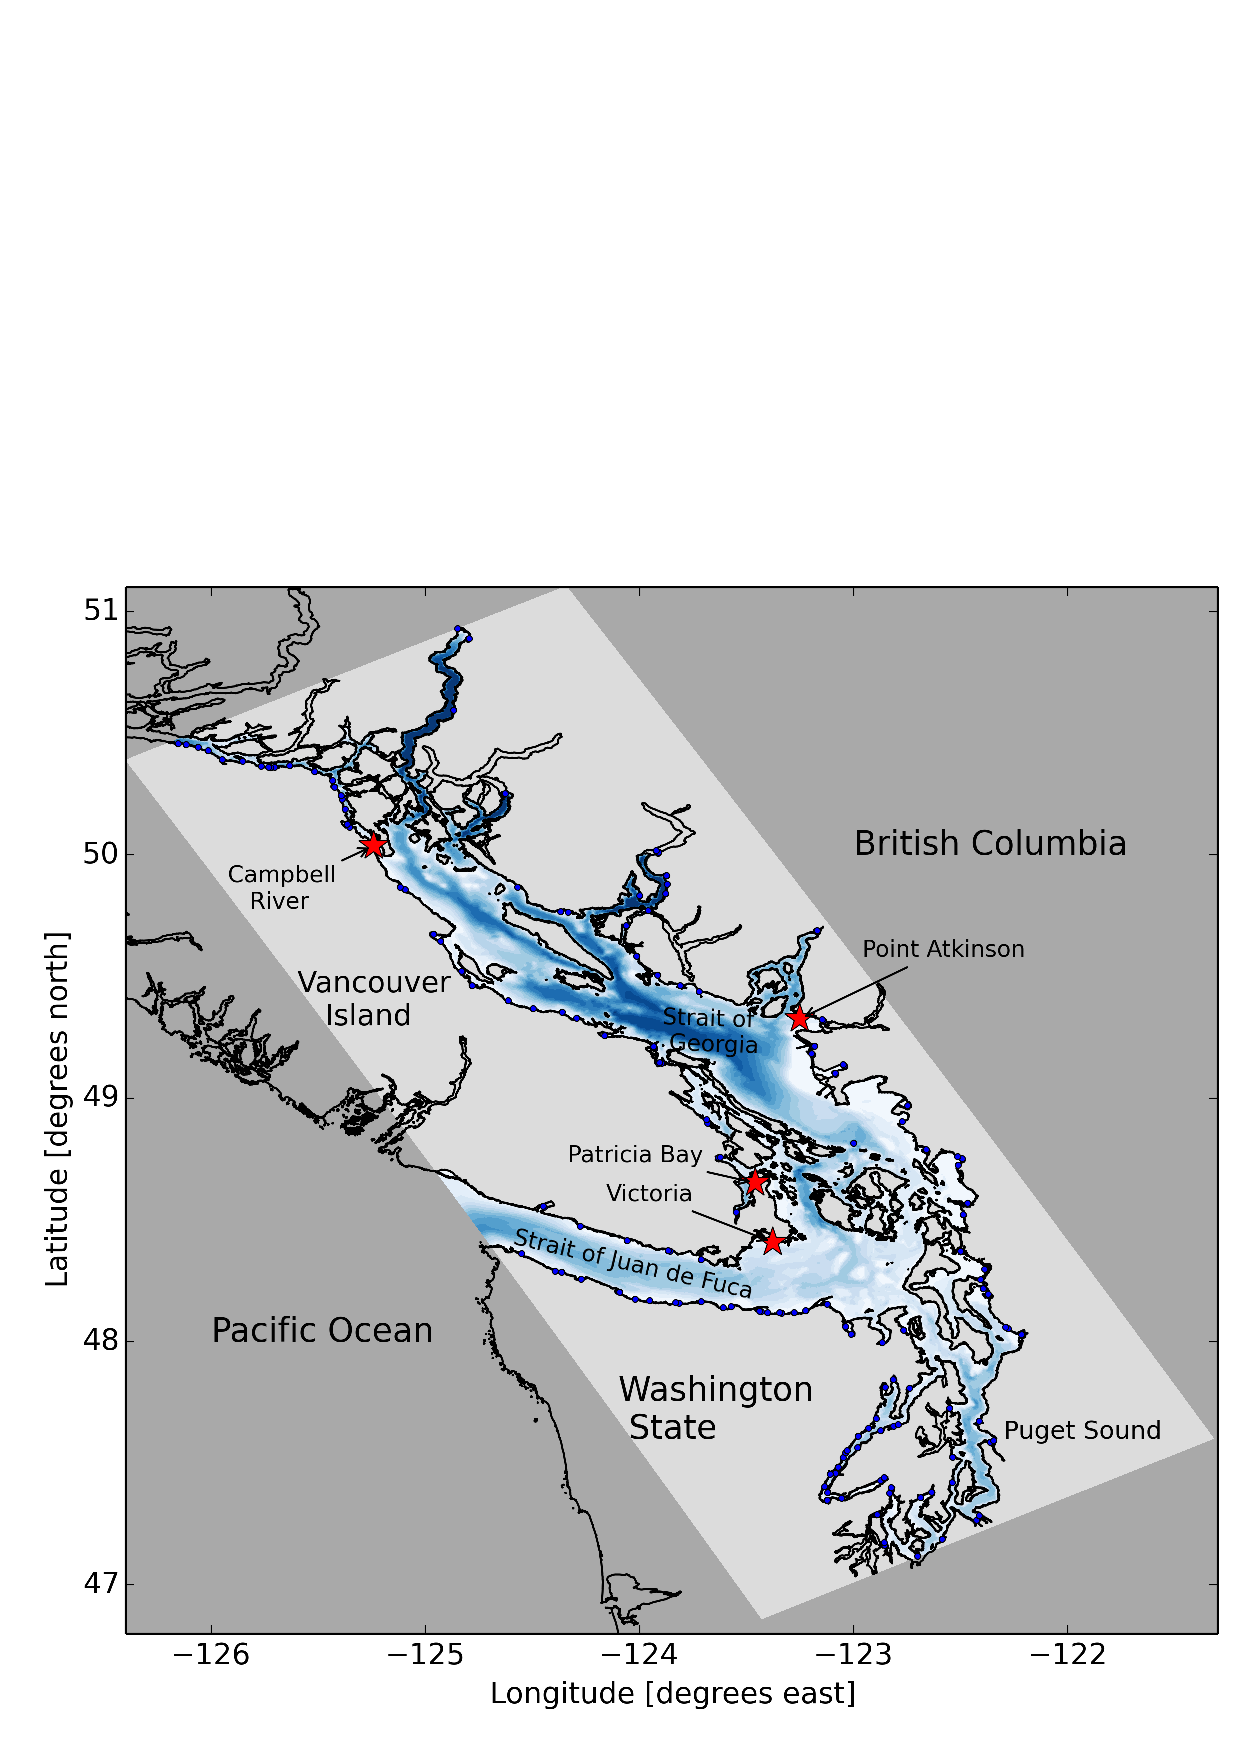
\includegraphics[scale=0.5]{Figures/bathy.png}
\caption{Model domain including bathymetry, rivers (*), and storm surge locations (o) of interest.}\label{fig:domain}
\end{figure}
%image needs some work: colour? labels for JdF, SoG, cities...

\subsection{Boundary conditions and sub-grid scale processes}
%lateral and bottom friction, open boundaries, eta surface
The model includes two open boundaries that connect to the Pacific Ocean, the western boundary of the Strait of Juan de Fuca as well as Johnstone Strait at the north, both of which are forced with eight tidal constituents, temperature and salinity climatologies, and the sea surface height anomaly. The details of these forcing conditions are described below. At coastal boundaries, the partial slip boundary condition, an approximation to no slip, is used. The partial slip boundary condition allows one to include the frictional effects of lateral boundaries without the restrictive resolution required to represent the lateral boundary layer under no slip conditions. A lateral eddy viscosity of 20 m $^2$ s $^{-1}$ parametrizes horizontal friction and the lateral eddy diffusivity is 20.5 m $^2$ s $^{-1}$ . At the ocean surface, meteorological conditions and fresh water input from rivers are included and described in more detail below. Bottom friction is represented by a quadratic law for the bottom momentum flux with drag coefficient $C_D = 5\times 10^{-3}$. Vertical turbulence and mixing is calculated through the $k-\epsilon$ configuration of the generic length scale (GLS) turbulence closure \citep{umlauf2003generic} with background vertical eddy viscosity and diffusivity set to $1\times10^{-4}$ and $1\times10^{-5}$ m$^2$ s$^{-1}$ respectively. Details on the NEMO implementation of the partial slip lateral boundary condition, quadratic bottom friction law, and GLS turbulence closure scheme are provided by \citet{madec2008nemo}.

In addition to the equations of motion, a prognostic equation for the sea surface height is solved at each time step. The inclusion the sea surface height equation requires a fairly restrictive time step due to the presence of high speed surface gravity waves. As such, the split-explicit time stepping algorithm is employed, where the free surface and barotropic equations are solved with a smaller time step than that used for the other variables. The model time step and barotropic time step are 10 s and 2 s respectively. 


\subsubsection{Tidal forcing} 
The model was forced by eight tidal constituents (K1 ,O1, P1, Q1, M2, K2, N2, S2) at the Juan de Fuca and Johnstone Strait boundaries. Tidal heights and currents at grid points along the Juan de Fuca boundary were extracted from Webtide, an online web prediction model for the northeast Pacific Ocean, which is based on work by \citet{foreman2000webtide}. The Johnstone Strait boundary was forced with current and elevation tidal harmonics measured and calculated by \citet{thomson1980johnstone} for the major M2 and K1 constituents. Additionally, O1 and S2 elevation harmonics from their measurements were employed. The remaining constituents were extrapolated from Webtide. 

\subsubsection{Temperature and salinity}
Temperature and salinity at the Juan de Fuca boundary were taken from a weekly climatology which was created from results from a model covering the Salish Sea and the west coast of Vancouver Island \citep{massonfine2012}.  Their results, originally on s-levels were interpolated onto z-levels and then onto the NEMO horizontal grid.  To prepare the climatology all years (1995-2008) were averaged and results, approximately every 15 days, were interpolated to a weekly climatology.

\subsubsection{Sea Surface Height}
Sea surface height at the mouth of Juan de Fuca was set using values from the Tofino tide gauge.  A monthly climatology was produced using daily averages from 2000-2010, binning them by month, averaging and setting the yearly mean to zero.  For the storm surge simulations, hourly variations in sea surface height were used.  These values are the Tofino tide gauge values, de-tided and with the zero reset as for the climatology. The storm surge simulations also used the sea surface height anomaly from Port Hardy, forced at the northern boundary in Johnstone Strait. 

\subsubsection{Open Boundary Conditions}

The model is relaxed to the forced temperature and salinity over the 10 grid points (about 5km) closest to the open boundaries, using a flow relaxation scheme \citep{engedahl1995use}. %other references?
The tidal forcing and sea surface height was used in the barotropic velocity forcing which used the NEMO Flather scheme \citep{flather1994storm, madec2008nemo}.
The baroclinic velocities at the boundary were set to be equal to the values inside the boundary (zero-gradient boundary conditions).  This scheme is not part of core NEMO.  Zero gradient conditions were chosen because the baroclinic velocity at the mouth of Juan de Fuca is primarily estuarine and thus set by density variations between inside and outside the domain.

\subsection{River forcing}
River input provides a significant volume of freshwater to the Salish Sea and can influence stratification, circulation and primary productivity. However, most rivers in the domain are not gauged so parameterisations were required to represent river flow. \citet{morrison2011rivers} provides a method for estimating freshwater runoff in the Salish Sea region based on precipitation. Monthly runoff volumes for each watershed for each year from 1970 to 2012 were acquired from \citet{morrison2011rivers}, as well as monthly averages. 

Freshwater runoff from each watershed was divided between the rivers in that watershed. The area drained by each river was estimated from Toporama maps by the Atlas of Canada and watershed maps available on the Washington State government website. The watersheds included in our model were Fraser (which represents approximately 44\% of the freshwater input into our domain), Skagit (12\%), East Vancouver Island (North and South) (12\%), Howe (7\%), Bute (7\%), Puget (6\%), Juan de Fuca (5\%), Jervis (4\%) and Toba (3\%). 

The monthly flow from each river was input as a point source in the three grid points closest to the surface at the model point closest to the mouth of each river. Incoming water was assumed to be fresh and at surface temperature. A total of 150 rivers were parameterised by this method. 

%we could show the location of all the rivers on the overall location map, or on a picture of our domain, since the rivers are on the edges of the domain so they won't block any bathymetry information

\subsection{Atmospheric forcing}
The ocean surface is forced with momentum and heat fluxes from a 33-km global atmospheric reforcasting model suitable for use in ocean modelling \citep{smith2013new}. Forecasts from the period of 2002-2011 are available. Additionally, the inverse barometric effect of the atmospheric pressure is included, an important consideration in storm surge modelling. 

\subsection{Initial conditions}
Initial conditions for temperature and salinity were taken from a CTD cast in the middle Strait of Georgia taken in Sept 2002 \citep{pawlowiczetal2007}.  Conditions were initially uniform horizontally.  Velocity was initialized at zero. 
%Merge with below?
%Perhaps image of spun-up stratification along Thalweg? Here or in model evaluation

\subsection{Spin-up}
The model was spun up for a 15.5 months from the initial conditions above, starting Sep 16, 2002, using atmospheric forcing from 2002-2003, climatological temperature and salinity and sea surface height at the boundaries, with tides and climatological river output.  All storm surge runs were started three days prior to the event of interest with zero initial velocities and sea surface height and a stratification profile from model spin up. The modelled sea surface height adjusted to forcing in less than one day. 

\section{Model Evaluation}\label{sec:model}

\subsection{Tidal evaluation}
The model was initially evaluated qualitatively by comparing patterns of tidal amplitude and phase to results from \citep{foreman1995tidal}. For example, the amphidromic dome around Victoria was produced in the $M_2$ results, as well as the monotonic increase in $K_1$ amplitude moving northwards along the Strait of Georgia. Initially, the Johnstone Strait boundary was closed, but modelled $M_2$ amplitudes were too small compared to measured amplitudes... TBC

%perhaps a nice contour map of M2 and K1 amps and phases goes here?

Once our model was reproducing observed tidal patterns, model results were quantitatively evaluated by comparing modelled harmonic constituents to measured harmonic constituents at tidal measuring stations throughout the domain. Comparisons were made using the complex difference (D), defined by \citep{foreman1995tidal} as:

\begin{equation}
D = [(A_0 \cos g_0 - A_m \cos g_m)^2 + (A_0 \sin g_0 - A_m \sin g_m)^2]^{1/2}
\end{equation}
where $A_0$, $A_m$, $g_0$ and $g_m$ are observed and modelled amplitudes and phases.

%perhaps a table of complex differences at tidal stations similar to Table 1 of Foreman et al (1995)  (such as the one produced by tidetools.calc_diffs_meas_mod) here?
%(would be cool to include the complex differences calculated at the VENUS nodes too)

Complex differences were less than ??cm at all stations in our domain, which was assumed to be acceptable for our purposes. 
%if it's favourable, we could compare our complex differences to Foreman et al (1995), who got an average of D=3cm for M2 and D=2.5cm for K1

\subsection{Stratification}

\section{Storm Surge Hind casts}\label{sec:storm}

\section{Conclusions}\label{sec:conclusions}


\bibliographystyle{chicago}
\bibliography{ref}

\end{document}

